\documentclass[12pt]{ctexart}

\usepackage[hmargin=3.18cm,vmargin=2.54cm]{geometry}
\usepackage{graphicx}
\usepackage{tabularx}
\usepackage{multicol}
\usepackage{ctex}
\usepackage{float}
\usepackage{amsmath}
\usepackage{subfigure}
\usepackage{fontspec}
\usepackage{setspace}

% 重定义有序列表样式
\renewcommand{\labelenumi}{(\arabic{enumi})}

\setmainfont{Times New Roman}

\ctexset{
  % 修改 part 标题样式
  part={
      format=\heiti\centering\zihao{3}
  },
  % 修改 section 标题样式
  section={   
    % 分隔符为 、
    name={,、},
    % 设置 section 标题为黑体、右对齐、小三号字
    format=\heiti\raggedright\zihao{-3}\bfseries,
    % 中文编号
    number={\chinese{section}},
    % 编号与标题名的间距
    aftername=\hspace{0.2em}
  },
  subsection={   
    % 无分隔符
    name={},
    % 设置 section 标题为宋体、右对齐、四号字
    format=\songti\raggedright\zihao{4}\bfseries,
    % 编号与标题名的间距
    aftername=\hspace{0.8em}
  },
  subsubsection={   
    name={},
    % 设置 section 标题为宋体、右对齐、小四号字
    format=\songti\raggedright\zihao{-4}\bfseries,
    % 编号与标题名的间距
    aftername=\hspace{0.8em}
  },
}

\begin{document}

\songti\zihao{-4}

\pagestyle{plain}

\thispagestyle{empty}
\part*{大标题}

\noindent{\textbf{摘要:}
  我是摘要,我是摘要。
}

\noindent{\textbf{关键词:}
  关键词\hspace{0.5em}
  关键词\hspace{0.5em}
  关键词
}
\newpage

\setcounter{page}{2}

\section{一级标题}
\subsection{二级标题}
\subsubsection{三级标题}

我是正文

I am body.

图片样例如图\ref{img_template}所示。

\begin{figure}[htbp!]
  \centering
  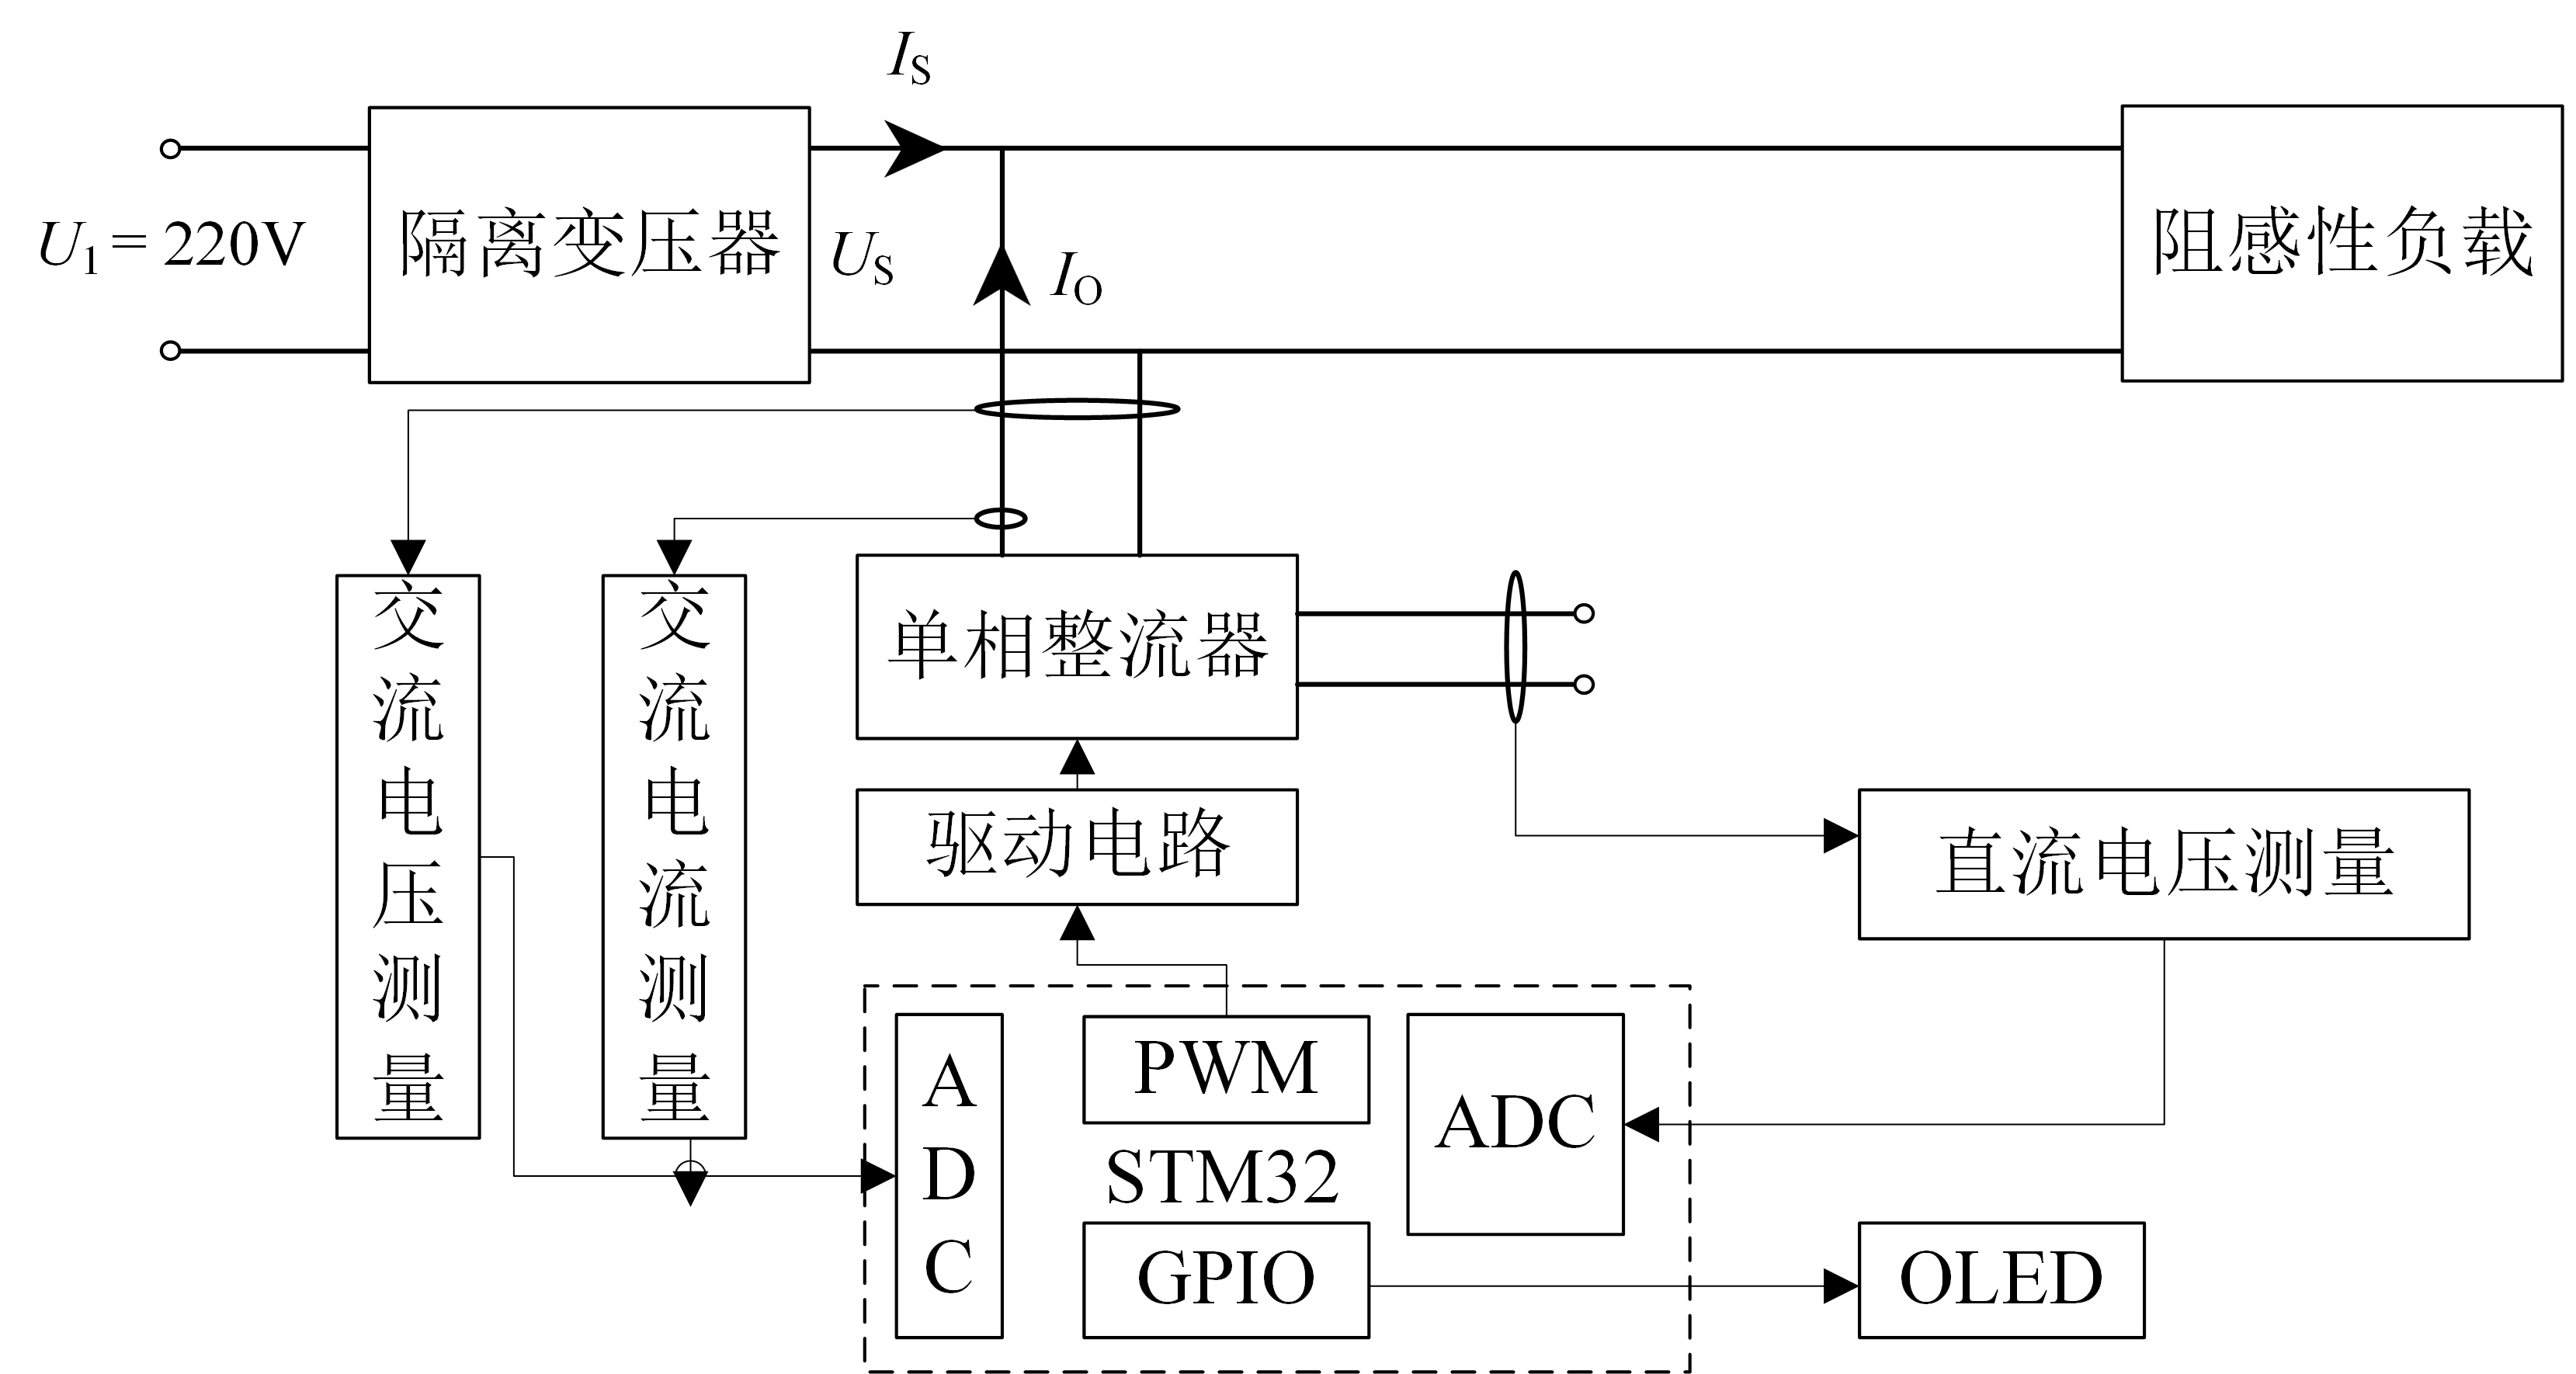
\includegraphics{img/template.png}
  \caption{我是图片样例}
  \label{img_template}
\end{figure}

我是行间下标的上一行。

行间下标长这样$U_{\rm S}$。

我是行间下标的下一行。

\end{document}

% 你可能会用到……

% 多张图并排

% \begin{figure}[htbp]
%   \begin{minipage}[t]{0.5\linewidth}
%     \centering
%     \includegraphics[width=0.9\linewidth]{img/figure_1.png}
%     \label{label_1}
%     \caption{figure 1}
%   \end{minipage}
%   \begin{minipage}[t]{0.5\linewidth}
%     \centering
%     \includegraphics[width=0.9\linewidth]{img/figure_2.png}
%     \label{label_2}
%     \caption{figure 2}
%   \end{minipage}
% \end{figure}